\section{Experimental Results}
\label{sec:experiments}

We finetune the model weights of the Imagenet-pretrained VGG-16 or ResNet-101
networks to adapt them to the semantic segmentation task in a straightforward
fashion, following the procedure of \cite{long2014fully}. We replace the
1000-way Imagenet classifier in the last layer with a classifier having as many
targets as the number of semantic classes of our task (including the background,
if applicable). Our loss function is the sum of cross-entropy terms for each
spatial position in the CNN output map (subsampled by 8 compared to the original
image). All positions and labels are equally weighted in the overall loss
function (except for unlabeled pixels which are ignored). Our targets are the
ground truth labels (subsampled by 8). We optimize the objective function with
respect to the weights at all network layers by the standard SGD procedure of
\cite{KrizhevskyNIPS2013}. We decouple the DCNN and CRF training stages,
assuming the DCNN unary terms are fixed when setting the CRF parameters.

We evaluate the proposed models on four challenging datasets: PASCAL VOC 2012,
PASCAL-Context, PASCAL-Person-Part, and Cityscapes. We first report the main
results of our conference version \cite{chen2014semantic} on PASCAL VOC 2012,
and move forward to latest results on all datasets.

%\textbf{Reproducibility} We have implemented the proposed methods by extending
%the Caffe framework \cite{jia2014caffe}. We share our code and models at a
%companion web site \url{http://liangchiehchen.com/projects/DeepLab.html}.

\subsection{PASCAL VOC 2012}

\textbf{Dataset:} The PASCAL VOC 2012 segmentation benchmark
\cite{everingham2014pascal} involves 20 foreground object classes and one
background class. The original dataset contains $1,464$ (\textit{train}),
$1,449$ (\textit{val}), and $1,456$ (\textit{test}) pixel-level labeled
images for training, validation, and testing, respectively. The dataset is
augmented by the extra annotations provided by \cite{hariharan2011semantic},
resulting in $10,582$ (\textit{trainaug}) training images. The performance
is measured in terms of pixel intersection-over-union (IOU) averaged across
the 21 classes.

\subsubsection{Results from our conference version}

We employ the VGG-16 network pre-trained on Imagenet, adapted for semantic
segmentation as described in Section~\ref{sec:convnet-hole}. We use a
mini-batch of 20 images and initial learning rate of $0.001$ ($0.01$
for the final classifier layer), multiplying the learning rate by 0.1 every
2000 iterations. We use momentum of $0.9$ and weight decay of $0.0005$.

After the DCNN has been fine-tuned on \textit{trainaug}, we cross-validate the
CRF parameters along the lines of \cite{krahenbuhl2011efficient}. We use default
values of $w_2 = 3$ and $\sigma_\gamma = 3$ and we search for the best values of
$w_1$, $\sigma_\alpha$, and $\sigma_\beta$ by cross-validation on 100 images
from \textit{val}. We employ a coarse-to-fine search scheme. The initial search
range of the parameters are $w_1 \in [3:6]$, $\sigma_\alpha \in [30:10:100]$ and
$\sigma_\beta \in [3:6]$ (MATLAB notation), and then we refine the search step
sizes around the first round's best values. We employ 10 mean field iterations.
%for all reported experiments.

\begin{table}[!t]
  \centering
  \addtolength{\tabcolsep}{2.5pt}
  \scalebox{0.97}{
  \begin{tabular}{c c c | c c | c}
    \toprule[0.2em]
    {\bf Kernel} & {\bf Rate} & {\bf FOV} & {\bf Params} & {\bf Speed} & {\bf bef/aft CRF} \\
    \toprule[0.2em]
    \by{7}{7}         &    4  & 224 & 134.3M & 1.44 & 64.38 / 67.64 \\
    \by{4}{4}         &    4  & 128 & 65.1M  & 2.90 & 59.80 / 63.74 \\
    \by{4}{4}         &    8  & 224 & 65.1M  & 2.90 & 63.41 / 67.14 \\
    \by{3}{3}         &   12  & 224 & 20.5M  & 4.84 & 62.25 / 67.64 \\
    \bottomrule[0.1em]
  \end{tabular}
  }
  \caption{Effect of Field-Of-View by adjusting the kernel size and atrous
    sampling rate $r$ at `fc6' layer. We show number of model parameters,
    training speed (img/sec), and \textit{val} set mean IOU before and after
    CRF. DeepLab-LargeFOV (kernel size \by{3}{3}, $r = 12$) strikes the best
    balance.}
  \label{tab:fov}
\end{table}

%% \begin{table}[!t]
%%   \centering
%%   \addtolength{\tabcolsep}{2.5pt}
%%   \begin{tabular}{l | c c}
%%     \toprule[0.2em]
%%     {\bf Method}      & {\bf no CRF} & {\bf with CRF}\\
%%     \toprule[0.2em]
%%     DeepLab     & 59.80 & 63.74 \\
%%     DeepLab-HC  & 61.30 & 65.21 \\
%%     DeepLab-7x7 & 64.38 & 67.64 \\
%%     DeepLab-LargeFOV & 62.25 & 67.64 \\
%%     DeepLab-HC-LargeFOV & 64.21 & 68.70 \\
%%     \bottomrule[0.1em]
%%   \end{tabular}
%%   \caption{Performance (mean IOU) of our proposed models on the PASCAL VOC 2012
%%     \textit{val} set with training in the \textit{trainaug} set. Hyper-column
%%     features, large field-of-view, and CRF improve performance.}
%%   \label{tb:valIOU}
%% \end{table}

%% \begin{figure}[!t]
%%   \centering
%%   \begin{tabular}{c c c c c}
%%     \includegraphics[height=0.11\linewidth]{fig/boundary_refine/vgg128noup_2007_003022.png} &
%%     \includegraphics[height=0.11\linewidth]{fig/boundary_refine/vgg128noup_2007_001284.png} &
%%     \includegraphics[height=0.11\linewidth]{fig/boundary_refine/vgg128noup_2007_001289.png} &
%%     \includegraphics[height=0.11\linewidth]{fig/boundary_refine/vgg128noup_2007_001311.png} &
%%     \includegraphics[height=0.11\linewidth]{fig/boundary_refine/vgg128noup_2009_000573.png} \\
%%     \includegraphics[height=0.11\linewidth]{fig/boundary_refine/vgg128ms_2007_003022.png} &
%%     \includegraphics[height=0.11\linewidth]{fig/boundary_refine/vgg128ms_2007_001284.png} &
%%     \includegraphics[height=0.11\linewidth]{fig/boundary_refine/vgg128ms_2007_001289.png} &
%%     \includegraphics[height=0.11\linewidth]{fig/boundary_refine/vgg128ms_2007_001311.png} &
%%     \includegraphics[height=0.11\linewidth]{fig/boundary_refine/vgg128ms_2009_000573.png} \\
%%   \end{tabular}
%%   \caption{Incorporating hyper-column features improves the boundary segmentation. We show the
%%     results obtained by DeepLab and DeepLab-HC in the first and second row, respectively.}
%%   \label{fig:msBoundary}
%% \end{figure}


%% \subsection{Multi-Scale Prediction}
%% \label{sec:multiscale}

%% Following the results of \cite{hariharan2014hypercolumns,
%%   long2014fully} we have also explored a multi-scale prediction method to
%% increase the boundary localization accuracy. Specifically, we attach
%% to the input image and the output of each of the first four max
%% pooling layers a two-layer MLP (first layer: 128 3x3 convolutional
%% filters, second layer: 128 1x1 convolutional filters) whose feature map
%% is concatenated to the main network's last layer feature map. The aggregate feature map
%% fed into the softmax layer is thus enhanced by 5 * 128 = 640
%% channels. We only adjust the newly added weights, keeping the other
%% network parameters to the values learned by the method of
%% Section~\ref{sec:convnets}. As discussed in the experimental section,
%% introducing these extra direct connections from fine-resolution layers
%% improves localization performance, yet the effect is not as dramatic
%% as the one obtained with the fully-connected CRF. 

\textbf{Field of View and CRF:}
 In \tabref{tab:fov}, we report experiments with DeepLab model variants that use
different field-of-view sizes, obtained by adjusting the kernel size and atrous
sampling rate $r$ in the `fc6' layer, as described in \secref{sec:convnet-hole}.
We start with a direct adaptation of VGG-16 net, using the original \by{7}{7}
kernel size and $r = 4$ (since we use no stride for the last two max-pooling
layers). This model yields performance of $67.64\%$ after CRF, but is relatively
slow ($1.44$ images per second during training). We have improved model speed to
$2.9$ images per second by reducing the kernel size to \by{4}{4}. We have
experimented with two such network variants with smaller ($r = 4$) and larger
($r = 8$) FOV sizes; the latter one performs better. Finally, we employ kernel
size \by{3}{3} and even larger atrous sampling rate ($r = 12$), also making the
network thinner by retaining a random subset of 1,024 out of the 4,096 filters
in layers `fc6' and `fc7'. The resulting model, DeepLab-CRF-LargeFOV, matches
the performance of the direct VGG-16 adaptation (\by{7}{7} kernel size, $r = 4$).
At the same time, DeepLab-LargeFOV is $3.36$ times faster and has significantly
fewer parameters (20.5M instead of 134.3M).

The CRF substantially boosts performance of all model variants, offering a 3-5\%
absolute increase in mean IOU.

%% \textbf{Hyper-column features:} We exploit the features from the intermediate layers,
%% similar to \cite{hariharan2014hypercolumns, long2014fully}. Specifically, we attach
%% to the input image and the output of each of the first four max pooling layers a
%% two-layer MLP (first layer: 128 \by{3}{3} convolutional filters, second layer:
%% 128 \by{1}{1} convolutional filters) whose feature map is concatenated to the main
%% network's last layer feature map. The aggregate feature map fed into the softmax
%% layer is thus enhanced by 5 * 128 = 640 channels. We only adjust the newly added
%% weights, keeping the other network parameters to the values learned before.
%% As shown in \tabref{tb:valIOU}, adding hyper-column features to our DeepLab model
%% (denoted as DeepLab-HC) brings about $1.5\%$ gain before CRF and about $4\%$ after
%% CRF. Qualitative comparison between DeepLab and DeepLab-HC in
%% \figref{fig:msBoundary} shows that hyper-column features improve accuracy close to
%% boundaries.

%% \textbf{Mean Pixel IOU along Object Boundaries:}
%% To quantify the accuracy of the proposed model near object boundaries, we evaluate
%% the segmentation accuracy with an experiment similar to \cite{kohli2009robust,
%% krahenbuhl2011efficient}. Specifically, we  use  the `void' label annotated in
%% \textit{val} set, which typically occurs around object boundaries. We compute the
%% mean IOU for those pixels that are located within a narrow band (called trimap) of
%% `void' labels. As shown in \figref{fig:IOUBoundary}, exploiting hyper-column
%% features and refining the segmentation results by a fully connected CRF
%% significantly improve the results around object boundaries. 

%% \begin{figure}[!t]
%% \centering
%% \resizebox{\columnwidth}{!}{
%%   \begin{tabular} {c c c}
%% %    \hspace{-0.5cm}\raisebox{2cm}
%%     \raisebox{1.0cm} {
%%     \begin{tabular}{c c}
%%       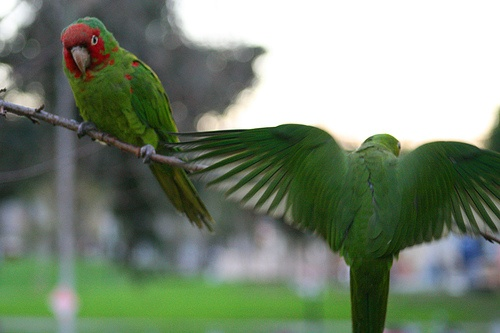
\includegraphics[height=0.1\linewidth]{fig/trimap/2007_000363.jpg} &
%%       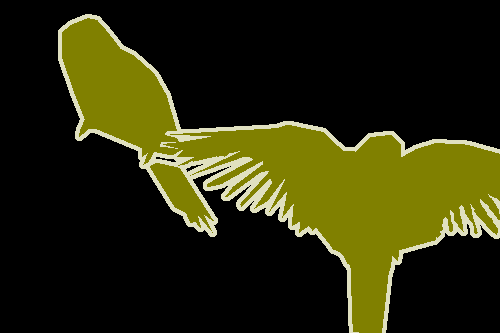
\includegraphics[height=0.1\linewidth]{fig/trimap/2007_000363.png} \\
%%       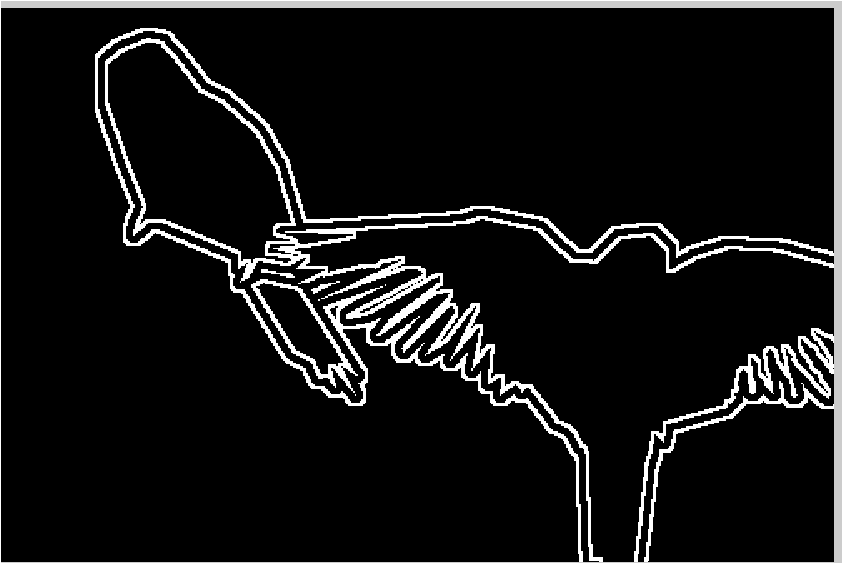
\includegraphics[height=0.1\linewidth]{fig/trimap/TrimapWidth2.pdf} &
%%       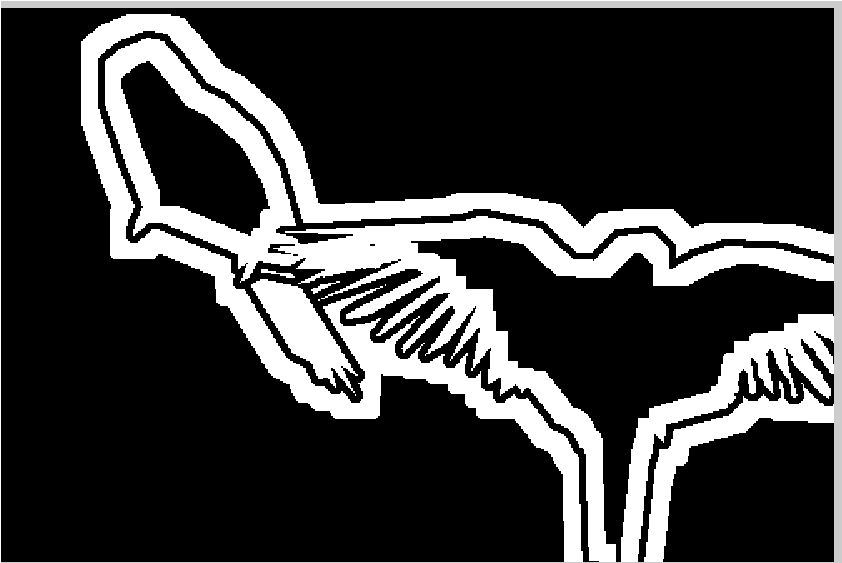
\includegraphics[height=0.1\linewidth]{fig/trimap/TrimapWidth10.pdf} \\
%%     \end{tabular} } &
%%     \includegraphics[height=0.25\linewidth]{fig/SegPixelAccWithinTrimap.pdf} &
%%     \includegraphics[height=0.25\linewidth]{fig/SegPixelIOUWithinTrimap.pdf} \\
%%     (a) & (b) & (c) \\
%%    \end{tabular}
%% }
%%   \caption{(a) Some trimap examples (top-left: image. top-right: ground-truth. bottom-left: trimap of 2 pixels. bottom-right: trimap of 10 pixels). Quality of segmentation result within a band around the object boundaries for the proposed methods. (b) Pixelwise accuracy. (c) Pixel mean IOU. 
%%     }  
%%   \label{fig:IOUBoundary}
%% \end{figure}

%Training time for 10 iterations: 139 sec (7x7) vs. 77 (4x4 hole=8) vs 67 (3x3 hole=12 ave) vs. 62 (3x3 hole=12). But we use batch size = 20 for 7x7 and 4x4, and batch size = 30 for 3x3. 69 sec for 4x4 (hole = 4)


%{\bf{Weighted loss: }} In PASCAL VOC 2012 dataset, most of the pixels are labeled as background in the ground truths. Weighting the loss function according to the class frequency has been employed, \eg \cite{farabet2013learning, mostajabi2014feedforward}, to overcome the label imbalance problem. Our experiments on VOC 2012 val set show that using a weighted loss function increases the mean class accuracy (the pixelwise accuracy averaged across classes), but does not improve the mean IOU in our model. 

%% \begin{figure}[t]
%%   \centering
%%   \begin{tabular}{c c}
%%     \includegraphics[height=0.55\linewidth]{fig/comparedWithFCN.pdf} &
%%     \includegraphics[height=0.55\linewidth]{fig/comparedWithRoomOut.pdf} \\
%%     (a) FCN-8s vs. DeepLab-CRF & (b) TTI-Zoomout-16 vs. DeepLab-CRF \\
%%   \end{tabular}
%%   \caption{Comparisons with state-of-the-art models on the val set. First row: images. Second row: ground truths. Third row: other recent models (Left: FCN-8s, Right: TTI-Zoomout-16). Fourth row: our DeepLab-CRF. Best viewed in color.}
%%   \label{fig:val_comparison}
%% \end{figure}

\textbf{Test set evaluation:} We have evaluated our DeepLab-CRF-LargeFOV model
on the PASCAL VOC 2012 official \textit{test} set. It achieves $70.3\%$ mean IOU
performance.

%% \begin{table}[t]
%%   \centering
%%   \addtolength{\tabcolsep}{2.5pt}
%%   \begin{tabular}{l | c}
%%     \toprule[0.2em]
%%     {\bf Method}      & {\bf mean IOU (\%)} \\
%%     \toprule[0.2em]
%% %    MSRA-CFM    & 61.8 \\
%% %    FCN-8s      & 62.2 \\
%% %    TTI-Zoomout-16 & 64.4 \\
%% %    \midrule \midrule
%%     DeepLab-CRF                 & 66.4 \\
%% %    DeepLab-HC-CRF             & 67.1 \\
%% %    DeepLab-CRF-7x7             & 70.3 \\
%%     DeepLab-CRF-LargeFOV        & 70.3 \\
%% %    DeepLab-CRF-MultiFOV        & 70.6 \\
%% %    DeepLab-HC-CRF-LargeFOV    & 71.6 \\
%%     \bottomrule[0.1em]
%%   \end{tabular}
%%   \caption{Performance of proposed models on the PASCAL VOC 2012 {\it test} set.}
%%   \label{tb:testIOU}
%% \end{table}


%% \begin{table*}[!tbp] %\scriptsize
%% \setlength{\tabcolsep}{3pt}
%% %\hspace{-1.8cm}
%% \resizebox{\columnwidth}{!}{
%% \begin{tabular}{|l||c*{20}{|c}||c|}
%% \hline 
%% Method         & bkg &  aero & bike & bird & boat & bottle& bus & car  &  cat & chair& cow  &table & dog  & horse & mbike& person& plant&sheep& sofa &train & tv   & mean \\
%% \hline \hline
%% MSRA-CFM       & -    & 75.7 & 26.7 & 69.5 & 48.8 & 65.6 & 81.0 & 69.2 & 73.3 & 30.0 & 68.7 & 51.5 & 69.1 & 68.1  & 71.7 & 67.5 & 50.4 & 66.5 & 44.4 & 58.9 & 53.5 & 61.8 \\
%% FCN-8s         & -    & 76.8 & 34.2 & 68.9 & 49.4 & 60.3 & 75.3 & 74.7 & 77.6 & 21.4 & 62.5 & 46.8 & 71.8 & 63.9  & 76.5 & 73.9 & 45.2 & 72.4 & 37.4 & 70.9 & 55.1 & 62.2 \\
%% TTI-Zoomout-16 & 89.8 & 81.9 & 35.1 & 78.2 & 57.4 & 56.5 & 80.5 & 74.0 & 79.8 & 22.4 & 69.6 & 53.7 & 74.0 & 76.0 & 76.6 & 68.8 & 44.3 & 70.2 & 40.2 & 68.9 & 55.3 & 64.4 \\
%% \hline
%% %\href{http://host.robots.ox.ac.uk:8080/anonymous/NTHWZK.html}
%% DeepLab-CRF    & 92.1 & 78.4 & 33.1 & 78.2 & 55.6 & 65.3 & 81.3 & 75.5 & 78.6 & 25.3 & 69.2 & 52.7 & 75.2 & 69.0  & 79.1 & 77.6 & 54.7 & 78.3 & 45.1 & 73.3 & 56.2 & 66.4 \\ 
%% %\href{http://host.robots.ox.ac.uk:8080/anonymous/UQUOMR.html}
%% DeepLab-HC-CRF & 92.6 & 80.4 & 36.8 & 77.4 & 55.2 & 66.4 & 81.5 & 77.5 & 78.9 & 27.1 & 68.2 & 52.7 & 74.3 & 69.6 & 79.4 & 79.0 & 56.9 & 78.8 & 45.2 & 72.7 & 59.3 &  67.1 \\
%% \href{http://host.robots.ox.ac.uk:8080/anonymous/EKRH3N.html}{DeepLab-CRF-7x7} & 92.8 & 83.9 & 36.6 & 77.5 & 58.4 & {\bf 68.0} & 84.6 & {\bf 79.7} & 83.1 & 29.5 & {\bf 74.6} & 59.3 & 78.9 & 76.0 & 82.1 & 80.6 & {\bf 60.3} & 81.7 & 49.2 & {\bf 78.0} & 60.7 & 70.3 \\
%% %\href{http://host.robots.ox.ac.uk:8080/anonymous/0KD2BO.html}
%% DeepLab-CRF-LargeFOV & 92.6 & 83.5 & 36.6 & {\bf 82.5} & 62.3 & 66.5 & {\bf 85.4} & 78.5 & {\bf 83.7} & 30.4 & 72.9 & {\bf 60.4} & 78.5 & 75.5 & 82.1 & 79.7 &  58.2 & 82.0 & 48.8 & 73.7 & 63.3 & 70.3 \\
%% %\href{http://host.robots.ox.ac.uk:8080/anonymous/UPP4XC.html}
%% DeepLab-HC-CRF-LargeFOV & {\bf 93.1} & {\bf 84.4} & {\bf 54.5} & 81.5 & {\bf 63.6} & 65.9 & 85.1 & 79.1 & 83.4 & {\bf 30.7} & 74.1 & 59.8 & {\bf 79.0} & {\bf 76.1} & {\bf 83.2} & {\bf 80.8} & 59.7 & {\bf 82.2} & {\bf 50.4} & 73.1 & {\bf 63.7} & {\bf 71.6} \\
%% \hline
%%  \end{tabular}
%% }
%%  \caption{Labeling IOU (\%) on the PASCAL VOC 2012 test set, using the trainval set for training.}
%%  \label{tab:voc2012}
%% \end{table*}



% \begin{figure}[ht]
%   \centering
%   \begin{tabular}{c c c | c c}
%     \includegraphics[height=0.12\linewidth]{fig/img/2007_002266.jpg} &
%     \includegraphics[height=0.12\linewidth]{fig/fcn8s/2007_002266.png} &
%     \includegraphics[height=0.12\linewidth]{fig/res_crf/2007_002266.png} &
%     \includegraphics[height=0.12\linewidth]{fig/SegPixelAccWithinTrimap_Berkeley.pdf} &
%     \includegraphics[height=0.12\linewidth]{fig/SegPixelIOUWithinTrimap_Berkeley.pdf} \\
%     (a) & (b) & (c) & (d) & (e)
%   \end{tabular}
%   \caption{(Left) Some comparisons with FCN-8S: (a) image; (b) FCN-8S; (c)
%     ms-crf. (d) Segmentation accuracy (pixelwise accuracy) within trimap. (e)
%     Segmentation accuracy (mean IOU) within trimap. {\color{red} TODO: change
%       legend. HELP: I cannot make them equally spaced....}} 
%   \label{fig:IOUBoundary}
% \end{figure}

%% \begin{figure*}[!htbp]
%%   \centering
%%   %\vspace{-1.cm}
%%   \scalebox{0.55} {
%%   \begin{tabular}{c c c | c c c | c c c}
%%     %\addtolength{\tabcolsep}{-6.5pt}
%%     \includegraphics[width=0.18\linewidth]{fig/voc12_val/img/2007_002094.jpg} &
%%     \includegraphics[width=0.18\linewidth]{fig/voc12_val/deeplab/res_none/2007_002094.png} &
%%     \includegraphics[width=0.18\linewidth]{fig/voc12_val/deeplab/res_crf/2007_002094.png} &
%%     \includegraphics[width=0.18\linewidth]{fig/voc12_val/img/2007_002719.jpg} &
%%     \includegraphics[width=0.18\linewidth]{fig/voc12_val/deeplab/res_none/2007_002719.png} &
%%     \includegraphics[width=0.18\linewidth]{fig/voc12_val/deeplab/res_crf/2007_002719.png} &
%%     \includegraphics[width=0.18\linewidth]{fig/voc12_val/img/2007_003957.jpg} &
%%     \includegraphics[width=0.18\linewidth]{fig/voc12_val/deeplab/res_none/2007_003957.png} &
%%     \includegraphics[width=0.18\linewidth]{fig/voc12_val/deeplab/res_crf/2007_003957.png} \\
%%     \includegraphics[width=0.18\linewidth]{fig/voc12_val/img/2007_003991.jpg} &
%%     \includegraphics[width=0.18\linewidth]{fig/voc12_val/deeplab/res_none/2007_003991.png} &
%%     \includegraphics[width=0.18\linewidth]{fig/voc12_val/deeplab/res_crf/2007_003991.png} &
%%     \includegraphics[width=0.18\linewidth]{fig/voc12_val/img/2008_001439.jpg} &
%%     \includegraphics[width=0.18\linewidth]{fig/voc12_val/deeplab/res_none/2008_001439.png} &
%%     \includegraphics[width=0.18\linewidth]{fig/voc12_val/deeplab/res_crf/2008_001439.png} &
%%     \includegraphics[width=0.18\linewidth]{fig/voc12_val/img/2008_004363.jpg} &
%%     \includegraphics[width=0.18\linewidth]{fig/voc12_val/deeplab/res_none/2008_004363.png} &
%%     \includegraphics[width=0.18\linewidth]{fig/voc12_val/deeplab/res_crf/2008_004363.png} \\
%%     \includegraphics[width=0.18\linewidth]{fig/voc12_val/img/2008_006229.jpg} &
%%     \includegraphics[width=0.18\linewidth]{fig/voc12_val/deeplab/res_none/2008_006229.png} &
%%     \includegraphics[width=0.18\linewidth]{fig/voc12_val/deeplab/res_crf/2008_006229.png} &
%%     \includegraphics[width=0.18\linewidth]{fig/voc12_val/img/2009_000421.jpg} &
%%     \includegraphics[width=0.18\linewidth]{fig/voc12_val/deeplab/res_none/2009_000421.png} &
%%     \includegraphics[width=0.18\linewidth]{fig/voc12_val/deeplab/res_crf/2009_000421.png} &
%%     \includegraphics[width=0.18\linewidth]{fig/voc12_val/img/2009_000412.jpg} &
%%     \includegraphics[width=0.18\linewidth]{fig/voc12_val/deeplab/res_none/2009_000412.png} &
%%     \includegraphics[width=0.18\linewidth]{fig/voc12_val/deeplab/res_crf/2009_000412.png} \\
%%     \includegraphics[width=0.18\linewidth]{fig/voc12_val/img/2010_001024.jpg} &
%%     \includegraphics[width=0.18\linewidth]{fig/voc12_val/deeplab/res_none/2010_001024.png} &
%%     \includegraphics[width=0.18\linewidth]{fig/voc12_val/deeplab/res_crf/2010_001024.png} &
%%     \includegraphics[width=0.18\linewidth]{fig/voc12_val/img/2010_001079.jpg} &
%%     \includegraphics[width=0.18\linewidth]{fig/voc12_val/deeplab/res_none/2010_001079.png} &
%%     \includegraphics[width=0.18\linewidth]{fig/voc12_val/deeplab/res_crf/2010_001079.png} &
%%     \includegraphics[width=0.18\linewidth]{fig/voc12_val/img/2007_002852.jpg} &
%%     \includegraphics[width=0.18\linewidth]{fig/voc12_val/deeplab/res_none/2007_002852.png} &
%%     \includegraphics[width=0.18\linewidth]{fig/voc12_val/deeplab/res_crf/2007_002852.png} \\
%%     \includegraphics[width=0.18\linewidth]{fig/voc12_val/img/2007_005331.jpg} &
%%     \includegraphics[width=0.18\linewidth]{fig/voc12_val/deeplab/res_none/2007_005331.png} &
%%     \includegraphics[width=0.18\linewidth]{fig/voc12_val/deeplab/res_crf/2007_005331.png} &
%%     \includegraphics[width=0.18\linewidth]{fig/voc12_val/img/2008_004654.jpg} &
%%     \includegraphics[width=0.18\linewidth]{fig/voc12_val/deeplab/res_none/2008_004654.png} &
%%     \includegraphics[width=0.18\linewidth]{fig/voc12_val/deeplab/res_crf/2008_004654.png} &
%%     \includegraphics[width=0.18\linewidth]{fig/voc12_val/img/2007_000129.jpg} &
%%     \includegraphics[width=0.18\linewidth]{fig/voc12_val/deeplab/res_none/2007_000129.png} &
%%     \includegraphics[width=0.18\linewidth]{fig/voc12_val/deeplab/res_crf/2007_000129.png} \\
%%     %\includegraphics[width=0.18\linewidth]{fig/voc12_val/img/2007_002619.jpg} &
%%     %\includegraphics[width=0.18\linewidth]{fig/voc12_val/deeplab/res_none/2007_002619.png} &
%%     %\includegraphics[width=0.18\linewidth]{fig/voc12_val/deeplab/res_crf/2007_002619.png} &
%%     \includegraphics[width=0.18\linewidth]{fig/voc12_val/img/2009_004504.jpg} &
%%     \includegraphics[width=0.18\linewidth]{fig/voc12_val/deeplab/res_none/2009_004504.png} &
%%     \includegraphics[width=0.18\linewidth]{fig/voc12_val/deeplab/res_crf/2009_004504.png} &
%%     \includegraphics[width=0.18\linewidth]{fig/voc12_val/img/2010_001069.jpg} &
%%     \includegraphics[width=0.18\linewidth]{fig/voc12_val/deeplab/res_none/2010_001069.png} &
%%     \includegraphics[width=0.18\linewidth]{fig/voc12_val/deeplab/res_crf/2010_001069.png} &
%%     \includegraphics[width=0.18\linewidth]{fig/voc12_val/img/2010_000038.jpg} &
%%     \includegraphics[width=0.18\linewidth]{fig/voc12_val/deeplab/res_none/2010_000038.png} &
%%     \includegraphics[width=0.18\linewidth]{fig/voc12_val/deeplab/res_crf/2010_000038.png} \\
%%     %% \hline
%%     %% \hline
%%     %% \includegraphics[width=0.18\linewidth]{fig/voc12_val/img/2007_000491.jpg} &
%%     %% \includegraphics[width=0.18\linewidth]{fig/voc12_val/deeplab/res_none/2007_000491.png} &
%%     %% \includegraphics[width=0.18\linewidth]{fig/voc12_val/deeplab/res_crf/2007_000491.png} &
%%     %% \includegraphics[width=0.18\linewidth]{fig/voc12_val/img/2007_000529.jpg} &
%%     %% \includegraphics[width=0.18\linewidth]{fig/voc12_val/deeplab/res_none/2007_000529.png} &
%%     %% \includegraphics[width=0.18\linewidth]{fig/voc12_val/deeplab/res_crf/2007_000529.png} &
%%     %% \includegraphics[width=0.14\linewidth]{fig/voc12_val/img/2007_000663.jpg} &
%%     %% \includegraphics[width=0.14\linewidth]{fig/voc12_val/deeplab/res_none/2007_000663.png} &
%%     %% \includegraphics[width=0.14\linewidth]{fig/voc12_val/deeplab/res_crf/2007_000663.png} \\    
%%     %% \includegraphics[width=0.18\linewidth]{fig/voc12_val/img/2007_000559.jpg} &
%%     %% \includegraphics[width=0.18\linewidth]{fig/voc12_val/deeplab/res_none/2007_000559.png} &
%%     %% \includegraphics[width=0.18\linewidth]{fig/voc12_val/deeplab/res_crf/2007_000559.png} &
%%     %% \includegraphics[width=0.18\linewidth]{fig/voc12_val/img/2007_000452.jpg} &
%%     %% \includegraphics[width=0.18\linewidth]{fig/voc12_val/deeplab/res_none/2007_000452.png} &
%%     %% \includegraphics[width=0.18\linewidth]{fig/voc12_val/deeplab/res_crf/2007_000452.png} &
%%     %% \includegraphics[width=0.18\linewidth]{fig/voc12_val/img/2007_002268.jpg} &
%%     %% \includegraphics[width=0.18\linewidth]{fig/voc12_val/deeplab/res_none/2007_002268.png} &
%%     %% \includegraphics[width=0.18\linewidth]{fig/voc12_val/deeplab/res_crf/2007_002268.png} \\
%%     (a) Image &
%%     (b) Before CRF &
%%     (c) After CRF &
%%     (a) Image &
%%     (b) Before CRF &
%%     (c) After CRF &
%%     (a) Image &
%%     (b) Before CRF &
%%     (c) After CRF \\
%%   \end{tabular}
%%   }
%%   %\vspace{-0.3cm}
%%   \caption{Visualization of some VOC 2012 \textit{val} results. For each row, we show
%%     the input image, the segmentation result before CRF, and the refined segmentation
%%     result after Fully Connected CRF (DeepLab-CRF). %% We show our failure modes in the last two rows.
%%   }
%%   \label{fig:ValResults}
%% \end{figure*}

% a block to the fc6 with hole = \{2,4,8,12\}. On the validation set, DeepLab has performance 63.67\% (1.42\% improvement over using one hole = 12, \ie, DeepLab-LargeFOV) and DeepLab-CRF yields 67.83\% (0.19\% improvement over DeepLab-CRF-LargeFOV). Similarly, we observe 0.3\% improvment over DeepLab-CRF-LargeFOV on the test set. The improvement of using multiple holes becomes marginal after employing dense CRF, which also has the effect of modeling long-range connection. 


\begin{figure*}[!htbp]
  \centering
  %\vspace{-1.cm}
  \scalebox{0.55} {
  \begin{tabular}{c}
    \includegraphics[width=1.8\linewidth]{fig/voc12_aspp/results.jpg}\\
  \end{tabular}
  }
  %\vspace{-0.3cm}
  \caption{PASCAL VOC 2012 \textit{val} results. Input image
    and our DeepLab results before/after CRF.}
  \label{fig:ValResults}
\end{figure*}


\subsubsection{Improvements after conference version of this work}
After the conference version of this work \cite{chen2014semantic}, we have
pursued three main improvements of our model, which we discuss below:
(1) different learning policy during training, (2) atrous spatial pyramid
pooling, and (3) employment of deeper networks and multi-scale processing.

\textbf{Learning rate policy:} We have explored different learning rate
policies when training DeepLab-LargeFOV. Similar to \cite{liu2015parsenet},
we also found that employing a ``poly'' learning rate policy (the learning
rate is multiplied by $(1-\frac{iter}{max\_iter})^{power}$) is more effective
than ``step'' learning rate (reduce the learning rate at a fixed step size).
As shown in \tabref{tab:val_poly}, employing ``poly'' (with $power = 0.9$)
and using the same batch size and same training iterations yields 1.17\% better
performance than employing ``step'' policy. Fixing the batch size and increasing
the training iteration to 10K improves the performance to 64.90\% (1.48\% gain);
however, the total training time increases due to more training iterations. We
then reduce the batch size to 10 and found that comparable performance is still
maintained (64.90\% \vs 64.71\%). In the end, we employ batch size = 10 and
20K iterations in order to maintain similar training time as previous ``step''
policy. Surprisingly, this gives us the performance of 65.88\% (3.63\%
improvement over ``step'') on \textit{val}, and 67.7\% on \textit{test},
compared to 65.1\% of the original ``step'' setting for DeepLab-LargeFOV before
CRF. We employ the ``poly'' learning rate policy for all experiments reported in
the rest of the paper.

\begin{table}[!t]
  \centering
  \addtolength{\tabcolsep}{2.5pt}
  \begin{tabular}{c c c c}
    \toprule[0.2 em]
    {\bf Learning policy} & {\bf Batch size} & {\bf Iteration} & {\bf mean IOU} \\
    \toprule[0.2em]
    step & 30 & 6K & 62.25 \\
    \midrule
    poly & 30 & 6K & 63.42 \\
    poly & 30 & 10K & 64.90 \\
    poly & 10 & 10K & 64.71 \\
    poly & 10 & 20K & 65.88 \\
    \bottomrule[0.1em]
  \end{tabular}
  \caption{PASCAL VOC 2012 \textit{val} set results (\%) (before CRF) as
    different learning hyper parameters vary. Employing ``poly'' learning
    policy is more effective than ``step'' when training DeepLab-LargeFOV.}
  \label{tab:val_poly}
\end{table}


\begin{figure}[!t]
  \centering
  \scalebox{0.85}{
  \begin{tabular}{c c}
    \includegraphics[width=0.2\linewidth]{./fig/spm/deeplab_largefov.pdf} &
    \includegraphics[height=4.5cm]{./fig/spm/deeplab_spm.pdf} \\
    {\scriptsize (a) DeepLab-LargeFOV} &
    {\scriptsize (b) DeepLab-ASPP} \\
  \end{tabular}
  }
  \caption{DeepLab-ASPP employs multiple filters with different rates to capture objects and context at multiple
    scales.}
  \label{fig:diff_hole}
\end{figure}

\textbf{Atrous Spatial Pyramid Pooling:} We have experimented with the proposed
Atrous Spatial Pyramid Pooling (ASPP) scheme, described in
\secref{sec:convnet-hole}. As shown in \figref{fig:diff_hole}, ASPP for VGG-16
employs several parallel fc6-fc7-fc8 branches. They all use \by{3}{3} kernels
but different atrous rates $r$ in the `fc6' in order to capture objects of
different size. In \tabref{tab:vgg_mfov}, we report results with several
settings:
(1) Our baseline LargeFOV model, having a single branch with $r=12$,
(2) ASPP-S, with four branches and smaller atrous rates ($r$ = \{2, 4, 8, 12\}), and
(3) ASPP-L, with four branches and larger rates ($r$ = \{6, 12, 18, 24\}).
For each variant we report results before and after CRF.
As shown in the table, ASPP-S yields 1.22\% improvement over the baseline
LargeFOV before CRF. However, after CRF both LargeFOV and ASPP-S perform similarly.
On the other hand, ASPP-L yields consistent improvements over the baseline LargeFOV
both before and after CRF. We evaluate on \textit{test} the proposed ASPP-L + CRF
model, attaining 72.6\%. We visualize the effect of the different schemes in
\figref{fig:aspp}.

\begin{table}[!t]
  \centering
  \addtolength{\tabcolsep}{0pt}
  \begin{tabular} {c | c c }
    \toprule[0.2em]
    {\bf Method} & {\bf before CRF} & {\bf after CRF} \\
    \toprule[0.2em]
    LargeFOV & 65.76 & 69.84 \\
    ASPP-S   & 66.98 & 69.73 \\
    ASPP-L   & 68.96 & 71.57 \\
    \bottomrule[0.1em]
  \end{tabular}
  \caption{Effect of ASPP on PASCAL VOC 2012 \textit{val} set
    performance (mean IOU) for VGG-16 based DeepLab model.
    {\bf LargeFOV}: single branch, $r = 12$.
    {\bf ASPP-S}: four branches, $r$ = \{2, 4, 8, 12\}.
    {\bf ASPP-L}: four branches, $r$ = \{6, 12, 18, 24\}.}
  \label{tab:vgg_mfov}
\end{table}

\begin{figure}
  \centering
  \begin{tabular}{c c c c}
    \includegraphics[width=0.21\linewidth]{fig/spm/img/2010_003947.jpg} &
    \includegraphics[width=0.21\linewidth]{fig/spm/vgg128_noup_pool3_20M_largewin3_newcode5/post_none/2010_003947.png} &
    \includegraphics[width=0.21\linewidth]{fig/spm/vgg128_noup_pool3_40M_largewin_spm_2/post_none/2010_003947.png} &    
    \includegraphics[width=0.21\linewidth]{fig/spm/vgg128_noup_pool3_40M_largewin_spm_3/post_none/2010_003947.png} \\
    \includegraphics[width=0.21\linewidth]{fig/spm/img/2010_003446.jpg} &
    \includegraphics[width=0.21\linewidth]{fig/spm/vgg128_noup_pool3_20M_largewin3_newcode5/post_none/2010_003446.png} &
    \includegraphics[width=0.21\linewidth]{fig/spm/vgg128_noup_pool3_40M_largewin_spm_2/post_none/2010_003446.png} &    
    \includegraphics[width=0.21\linewidth]{fig/spm/vgg128_noup_pool3_40M_largewin_spm_3/post_none/2010_003446.png} \\
    (a) Image &
    (b) LargeFOV &
    (c) ASPP-S &
    (d) ASPP-L \\
  \end{tabular}
  \caption{Qualitative segmentation results with ASPP compared to the baseline
    LargeFOV model. The \textbf{ASPP-L} model, employing multiple {\it large}
    FOVs can successfully capture objects as well as image context at multiple
    scales.}
  \label{fig:aspp}
\end{figure}


\begin{table}[!t]
  \centering
  \addtolength{\tabcolsep}{-1pt}
  \begin{tabular} {c c c c c c | c}
    \toprule[0.2em]
    {\bf MSC} & {\bf COCO} & {\bf Aug} & {\bf LargeFOV} & {\bf ASPP} & {\bf CRF} & {\bf mIOU} \\
    \toprule[0.2em]
    %\multicolumn{7}{l}{\it VGG-16 net}  \\
    %DeepLab-LargeFOV \cite{chen2014semantic} & 62.25 \\
    %DeepLab-LargeFOV-Max \cite{chen2015attention}& 67.79 \\
    %DeepLab-LargeFOV-COCO \cite{papandreou2015weakly} & 67.58 \\
    %DeepLab \cite{chen2015attention} & \check & \check & & \check 70.06 \\
    %\midrule
    %\multicolumn{7}{l}{\it ResNet-101} & \\
    & & & & & & 68.72 \\
    \checkmark & & & & & & 71.27 \\
    \checkmark & \checkmark & & & & & 73.28 \\
%    DeepLab-COCO & 73.50 \\
    \checkmark & \checkmark & \checkmark & & & & 74.87 \\
    %DeepLab-CRF-Max-COCO+ & & & & & & 75.95 \\
    \checkmark & \checkmark & \checkmark & \checkmark & & & 75.54 \\
    \checkmark & \checkmark & \checkmark & & \checkmark & & 76.35 \\
    \checkmark & \checkmark & \checkmark & & \checkmark & \checkmark & 77.69 \\
    \bottomrule[0.1em]
  \end{tabular}
  \caption{Employing ResNet-101 for DeepLab on PASCAL VOC 2012 {\it val} set.
    {\bf MSC}: Employing mutli-scale inputs with max fusion.
    {\bf COCO}: Models pretrained on MS-COCO.
    {\bf Aug}: Data augmentation by randomly rescaling inputs.}
  \label{tab:resnet_val}
\end{table}

\textbf{Deeper Networks and Multiscale Processing:} We have experimented
building DeepLab around the recently proposed residual net ResNet-101
\cite{he2015deep} instead of VGG-16. Similar to what we did for VGG-16 net,
we re-purpose ResNet-101 by atrous convolution, as described in
\secref{sec:convnet-hole}. On top of that, we adopt several other features,
following recent work of \cite{farabet2013learning, papandreou2015weakly,
  zheng2015conditional, liu2015semantic, lin2015efficient, chen2015attention,
  kokkinos2016pushing}: (1) Multi-scale inputs: We separately feed to the
DCNN images at scale = \{0.5, 0.75, 1\}, fusing their score maps by taking
the maximum response across scales for each position separately
\cite{chen2015attention}. (2) Models pretrained on MS-COCO
\cite{lin2014microsoft}. (3) Data augmentation by randomly scaling the input
images (from 0.5 to 1.5) during training. In \tabref{tab:resnet_val}, we
evaluate how each of these factors, along with LargeFOV and atrous spatial
pyramid pooling (ASPP), affects \textsl{val} set performance.
Adopting ResNet-101 instead of VGG-16 significantly improves DeepLab performance
(\eg, our simplest ResNet-101 based model attains 68.72\%, compared to 65.76\%
of our DeepLab-LargeFOV VGG-16 based variant, both before CRF). Multiscale
fusion \cite{chen2015attention} brings extra 2.55\% improvement, while
pretraining the model on MS-COCO gives another 2.01\% gain. Data augmentation
during training is effective (about 1.6\% improvement). Employing LargeFOV
(adding an atrous convolutional layer on top of ResNet, with \by{3}{3} kernel
and rate = 12) is beneficial (about 0.6\% improvement). Further 0.8\%
improvement is achieved by atrous spatial pyramid pooling (ASPP).
Post-processing our best model by dense CRF yields performance of 77.69\%.

%We report the performance on the validation set in \tabref{tab:resnet_val}. As shown in the table, adopting ResNet-101 for DeepLab significantly outperform the performance when employing VGG-16 net. 
%Following the recent work of , we employ as input an image pyramid (specifically, images with scale = \{0.5, 0.75, 1\}). Similar to \cite{chen2015attention}, we also use extra supervision and max-pooling to merge the results from all the scales. The method proposed by \cite{chen2015attention} exploits the multi-scale features (by scaling the input images) more efficiently while only one-step end-to-end training of the DeepLab part is required. Please refer to \cite{chen2015attention} for details.
%We denote the model, adopting the multi-scale inputs and max-pooling to merge the results \cite{chen2015attention}, as DeepLab-Max. In that case, DeepLab-Max (ResNet-101) outperform DeepLab-LargeFOV-Max (VGG-16) by 3.48\%. Pretraining the model on the MS-COCO dataset \cite{lin2014microsoft} gives extra 2\% improvement (denoted as DeepLab-Max-COCO). Similar to \cite{lin2015efficient}, augmenting the dataset by randomly scaling the input images (from 0.5 to 1.5) during training brings about 1.6\% more improvement (denoted as DeepLab-Max-COCO+). After incorporating dense CRF as post processing, our model, DeepLab-CRF-Max-COCO+, achieves the performance of 75.95\% on the validation set. Note that we observe adopting ResNet-52 \cite{he2015deep} has worse performance than ResNet-101, while ResNet-152 has similar performance to ResNet-101 but with longer processing time for each image. We, thus, adopt ResNet-101 for all the experiments. 

\textbf{Qualitative results:} We provide qualitative visual comparisons of DeepLab's
results (our best model variant) before and after CRF in \figref{fig:ValResults}.
The visualization results obtained by DeepLab before CRF already yields excellent
segmentation results, while employing the CRF further improves the performance by
removing false positives and refining object boundaries. 


%We conduct the majority of our evaluations
%on the \textit{val} set, training our model on the \textit{trainaug} set.
%We note that the work of
%\cite{krahenbuhl2011efficient} improved the $27.6\%$ result of TextonBoost
%\cite{shotton2009textonboost} to $29.1\%$, which makes the improvement we report
%here (from $59.8\%$ to $63.7\%$) all the more impressive.
%We provide qualitative visual comparisons of DeepLab's
%results before and after CRF in \figref{fig:ValResults}. Employing the CRF
%leads to significant qualitative improvements, allowing the model to accurately
%capture intricate object boundaries.

\textbf{Test set results:} We have submitted the result of our final best model
to the official server, obtaining \textit{test} set performance of 79.7\%, as
shown in \tabref{tab:res_testset}. The model substantially outperforms previous
DeepLab variants (\eg, DeepLab-LargeFOV with VGG-16 net) and is currently the
top performing method on the PASCAL VOC 2012 segmentation leaderboard. 

%, and is comparable with concurrent work \cite{wu2016high} which further employs on-line hard example mining. 
%% We have observed a marginal further 0.3\% improvement by adopting an ensemble
%% approach \cite{szegedy2014going, he2015deep, noh2015learning, liu2015semantic}.
%% Averaging the results of two ASPP models (one trained on \textit{trainval} and
%% another on \textit{trainvalaug}), we achieve 79.6\% on the test set. Integrating
%% into our model other advanced methods (\eg, joint training of DCNN and CRF
%% \cite{zheng2015conditional,arnab2015higher}, four step training \cite{liu2015semantic},
%% and non-linear pairwise term \cite{lin2015efficient}) could lead to further improvements.

\begin{table}[!th]
  \centering
  \addtolength{\tabcolsep}{2.5pt}
  \begin{tabular}{l | c}
    \toprule[0.2 em]
    {\bf Method} & {\bf mIOU} \\
    \toprule[0.2 em]
    %DeepLab-LargeFOV-COCO (VGG-16 net) \cite{papandreou2015weakly} & 68.9\\
    %\midrule
    DeepLab-CRF-LargeFOV-COCO \cite{papandreou2015weakly} & 72.7\\
    MERL\_DEEP\_GCRF \cite{Vemulapalli2016Gaussian} & 73.2 \\
    CRF-RNN \cite{zheng2015conditional} & 74.7 \\
    POSTECH\_DeconvNet\_CRF\_VOC \cite{noh2015learning} & 74.8 \\
    BoxSup \cite{dai2015boxsup} & 75.2 \\
    Context + CRF-RNN \cite{yu2015multi} & 75.3 \\
    $QO_4^{mres}$ \cite{chandra2016fast} & 75.5 \\
    DeepLab-CRF-Attention \cite{chen2015attention} & 75.7 \\
    CentraleSuperBoundaries++ \cite{kokkinos2016pushing} & 76.0 \\
    DeepLab-CRF-Attention-DT  \cite{chen2015semantic} & 76.3 \\
    H-ReNet + DenseCRF \cite{yan2016combining} & 76.8 \\
    LRR\_4x\_COCO \cite{ghiasi2016laplacian} & 76.8 \\
    DPN \cite{liu2015semantic} & 77.5 \\
    Adelaide\_Context \cite{lin2015efficient} & 77.8 \\
    Oxford\_TVG\_HO\_CRF \cite{arnab2015higher} & 77.9 \\
    Context CRF + Guidance CRF \cite{Shen2016Fast} & 78.1 \\
    Adelaide\_VeryDeep\_FCN\_VOC \cite{wu2016bridging} & 79.1 \\
    \midrule
    \href{http://host.robots.ox.ac.uk:8080/anonymous/FLHY8R.html}{DeepLab-CRF (ResNet-101)} & 79.7 \\
%    \href{http://host.robots.ox.ac.uk:8080/anonymous/SV4ESR.html}{Ensemble DeepLab-CRF (ResNet-101)} & 79.6 \\
    \bottomrule[0.1 em]
  \end{tabular}
  \caption{Performance on PASCAL VOC 2012 {\it test} set. We have added some
    results from recent arXiv papers on top of the official leadearboard results.}
  \label{tab:res_testset}
\end{table}

\textbf{VGG-16 \vs ResNet-101:} We have observed that DeepLab based on ResNet-101 \cite{he2015deep}
delivers better segmentation results along object boundaries than employing VGG-16 \cite{simonyan2014very}, as
visualized in \figref{fig:res_vs_vgg_results}. We think the identity mapping \cite{he2016identity} of ResNet-101
has similar effect as hyper-column features \cite{hariharan2014hypercolumns}, which exploits the features from
the intermediate layers to better localize boundaries. We further quantize this effect in \figref{fig:IOUBoundary} within the
``trimap'' \cite{kohli2009robust, krahenbuhl2011efficient} (a narrow band along object boundaries). As shown in
the figure, employing ResNet-101 before CRF has almost the same accuracy along object boundaries as employing
VGG-16 in conjunction with a CRF. Post-processing the ResNet-101 result with a CRF further improves the segmentation
result.

\begin{figure}[!t]
  \centering
  %\vspace{-1.cm}
  \scalebox{0.85} {
  \begin{tabular}{c @{\hskip 5pt} c @{\hskip 5pt} c @{\hskip 5pt} c @{\hskip 5pt} c}
    %%\addtolength{\tabcolsep}{10pt}
    %% \includegraphics[width=0.18\linewidth]{fig/res_vs_vgg/resnet101_noup_pool3_14/img/2007_000129.jpg} &
    %% \includegraphics[width=0.18\linewidth]{fig/res_vs_vgg/vgg128_noup_pool3_20M_largewin3_newcode5/res_none/2007_000129.png} &
    %% \includegraphics[width=0.18\linewidth]{fig/res_vs_vgg/vgg128_noup_pool3_20M_largewin3_newcode5/res_crf/2007_000129.png} &
    %% \includegraphics[width=0.18\linewidth]{fig/res_vs_vgg/resnet101_noup_pool3_14/res_none/2007_000129.png} &
    %% \includegraphics[width=0.18\linewidth]{fig/res_vs_vgg/resnet101_noup_pool3_14/res_crf/2007_000129.png} \\

    %% \includegraphics[width=0.18\linewidth]{fig/res_vs_vgg/resnet101_noup_pool3_14/img/2008_006874.jpg} &
    %% \includegraphics[width=0.18\linewidth]{fig/res_vs_vgg/vgg128_noup_pool3_20M_largewin3_newcode5/res_none/2008_006874.png} &
    %% \includegraphics[width=0.18\linewidth]{fig/res_vs_vgg/vgg128_noup_pool3_20M_largewin3_newcode5/res_crf/2008_006874.png} &
    %% \includegraphics[width=0.18\linewidth]{fig/res_vs_vgg/resnet101_noup_pool3_14/res_none/2008_006874.png} &
    %% \includegraphics[width=0.18\linewidth]{fig/res_vs_vgg/resnet101_noup_pool3_14/res_crf/2008_006874.png} \\

    \includegraphics[width=0.21\linewidth]{fig/res_vs_vgg/resnet101_noup_pool3_14/img/2007_001311.jpg} &
    \includegraphics[width=0.21\linewidth]{fig/res_vs_vgg/vgg128_noup_pool3_20M_largewin3_newcode5/res_none/2007_001311.png} &
    \includegraphics[width=0.21\linewidth]{fig/res_vs_vgg/vgg128_noup_pool3_20M_largewin3_newcode5/res_crf/2007_001311.png} &
    \includegraphics[width=0.21\linewidth]{fig/res_vs_vgg/resnet101_noup_pool3_14/res_none/2007_001311.png} &
    \includegraphics[width=0.21\linewidth]{fig/res_vs_vgg/resnet101_noup_pool3_14/res_crf/2007_001311.png} \\

    \includegraphics[width=0.21\linewidth]{fig/res_vs_vgg/resnet101_noup_pool3_14/img/2011_000455.jpg} &
    \includegraphics[width=0.21\linewidth]{fig/res_vs_vgg/vgg128_noup_pool3_20M_largewin3_newcode5/res_none/2011_000455.png} &
    \includegraphics[width=0.21\linewidth]{fig/res_vs_vgg/vgg128_noup_pool3_20M_largewin3_newcode5/res_crf/2011_000455.png} &
    \includegraphics[width=0.21\linewidth]{fig/res_vs_vgg/resnet101_noup_pool3_14/res_none/2011_000455.png} &
    \includegraphics[width=0.21\linewidth]{fig/res_vs_vgg/resnet101_noup_pool3_14/res_crf/2011_000455.png} \\

    {\scriptsize Image} &
    {\scriptsize VGG-16 Bef.} &
    {\scriptsize VGG-16 Aft.} &
    {\scriptsize ResNet Bef.} &
    {\scriptsize ResNet Aft.} \\
  \end{tabular}
  }
  %\vspace{-0.3cm}
  \caption{DeepLab results based on VGG-16 net or ResNet-101 before and after CRF.
    The CRF is critical for accurate prediction along object boundaries with VGG-16, whereas
    ResNet-101 has acceptable performance even before CRF.}
  \label{fig:res_vs_vgg_results}
\end{figure}

\begin{figure}[!t]
\centering
\resizebox{\columnwidth}{!}{
  \begin{tabular} {c c}
%    \hspace{-0.5cm}\raisebox{2cm}
    \raisebox{1cm} {
    \begin{tabular}{c c}
      \includegraphics[height=0.1\linewidth]{fig/trimap/2007_000363.jpg} &
      \includegraphics[height=0.1\linewidth]{fig/trimap/2007_000363.png} \\
      \includegraphics[height=0.1\linewidth]{fig/trimap/TrimapWidth2.pdf} &
      \includegraphics[height=0.1\linewidth]{fig/trimap/TrimapWidth10.pdf} \\
    \end{tabular} } &
    \includegraphics[height=0.25\linewidth]{fig/res_vs_vgg/SegPixelIOUWithinTrimap_ResVsVGG} \\
    (a) & (b) \\
   \end{tabular}
}
  \caption{(a) Trimap examples (top-left: image. top-right: ground-truth. bottom-left: trimap of 2 pixels.
    bottom-right: trimap of 10 pixels). (b) Pixel mean IOU as a function of the band width around the
    object boundaries when employing VGG-16 or ResNet-101 before and after CRF.}
  \label{fig:IOUBoundary}
\end{figure}


\subsection{PASCAL-Context}
\label{exp:pascal_context}

\begin{figure*}[!t]
  \centering
  %\vspace{-1.cm}
  \scalebox{0.9} {
  \begin{tabular}{c}
    \includegraphics[width=1\linewidth]{fig/pascal_context/results.jpg} \\
  \end{tabular}
  }
  \caption{PASCAL-Context results. Input image, ground-truth,
    and our DeepLab results before/after CRF.}
  \label{fig:pascal_context_val_results}
\end{figure*}

\begin{table}[!t]
  \centering
  \addtolength{\tabcolsep}{-3pt}
  \begin{tabular} {l c c c c c c | c}
    \toprule[0.2 em]
    {\bf Method} & {\bf MSC} & {\bf COCO} & {\bf Aug} & {\bf LargeFOV} & {\bf ASPP} & {\bf CRF} & {\bf mIOU} \\
    \toprule[0.2 em]
    \multicolumn{7}{l}{\it VGG-16} & \\
    DeepLab \cite{chen2014semantic}& & & &\checkmark & & & 37.6 \\
    DeepLab \cite{chen2014semantic}& & & &\checkmark & & \checkmark  &  39.6 \\
    \midrule
    \multicolumn{7}{l}{\it ResNet-101} & \\
    DeepLab & & & & & & &  39.6 \\
    DeepLab &\checkmark & & \checkmark & & & &  41.4 \\
    DeepLab &\checkmark &\checkmark & \checkmark & & & &  42.9 \\
    DeepLab &\checkmark &\checkmark & \checkmark & \checkmark & & & 43.5 \\
    DeepLab &\checkmark &\checkmark & \checkmark & & \checkmark & & 44.7 \\
    DeepLab &\checkmark &\checkmark & \checkmark & & \checkmark & \checkmark & 45.7 \\
%    DeepLab-CRF-Max (ResNet-101) & 43.1 \\
%    DeepLab-CRF-Max-COCO (ResNet-101) & 44.5 \\
    \midrule \midrule
    $O_2P$ \cite{carreira2012semantic}& & & & & &  & 18.1 \\
    CFM \cite{dai2014convolutional}& & & & & &  & 34.4 \\
    FCN-8s \cite{long2014fully}& & & & & &  & 37.8 \\
    CRF-RNN \cite{zheng2015conditional}& & & & & &  & 39.3 \\
    ParseNet \cite{liu2015parsenet}& & & & & &  & 40.4 \\
    BoxSup \cite{dai2015boxsup}& & & & & &  & 40.5 \\
    HO\_CRF \cite{arnab2015higher}& & & & & &  & 41.3 \\
    Context \cite{lin2015efficient}& & & & & &  & 43.3 \\
    VeryDeep \cite{wu2016bridging}& & & & & &  & 44.5 \\
    \bottomrule[0.1 em]
  \end{tabular}
  \caption{Comparison with other state-of-art methods on PASCAL-Context dataset.}
  \label{tab:pascal_context}
\end{table}

\textbf{Dataset:} The PASCAL-Context dataset \cite{mottaghi2014role} provides
detailed semantic labels for the whole scene, including both object (\eg, person)
and stuff (\eg, sky). Following \cite{mottaghi2014role}, the proposed models are
evaluated on the most frequent 59 classes along with one background category.
The training set and validation set contain 4998 and 5105 images.

\textbf{Evaluation:} We report the evaluation results in \tabref{tab:pascal_context}.
Our VGG-16 based LargeFOV variant yields 37.6\% before and 39.6\% after CRF.
Repurposing the ResNet-101 \cite{he2015deep} for DeepLab improves 2\% over the
VGG-16 LargeFOV. Similar to \cite{chen2015attention}, employing multi-scale inputs
and max-pooling to merge the results improves the performance to 41.4\%.
Pretraining the model on MS-COCO brings extra 1.5\% improvement.
Employing atrous spatial pyramid pooling is more effective than LargeFOV.
After further employing dense CRF as post processing, our final model
yields 45.7\%, outperforming the current state-of-art method
\cite{lin2015efficient} by 2.4\% without using their non-linear pairwise term. Our final
model is slightly better than the concurrent work \cite{wu2016bridging} by 1.2\%, which also employs
atrous convolution to repurpose the residual net of \cite{he2015deep} for semantic segmentation.

\textbf{Qualitative results:} We visualize the segmentation results of our best
model with and without CRF as post processing in
\figref{fig:pascal_context_val_results}. DeepLab before CRF can already predict
most of the object/stuff with high accuracy. Employing CRF, our model is able to
further remove isolated false positives and improve the prediction along
object/stuff boundaries.

\subsection{PASCAL-Person-Part}
\label{exp:pascal_person_part}

\begin{figure*}[!th]
  \centering
  %\vspace{-1.cm}
  \scalebox{0.9} {
  \begin{tabular}{c}
    \includegraphics[width=1.\linewidth]{fig/voc10_part/results.jpg} \\
  \end{tabular}
  }
  \caption{PASCAL-Person-Part results. Input image, ground-truth,
    and our DeepLab results before/after CRF.}
  \label{fig:voc10_part_val_results}
\end{figure*}

\begin{table}[!t]
  \centering
  \addtolength{\tabcolsep}{-3pt}
  \begin{tabular} {l  c c c c c c | c}
    \toprule[0.2 em]
    {\bf Method} & {\bf MSC} & {\bf COCO} & {\bf Aug} & {\bf LFOV} & {\bf ASPP} & {\bf CRF} & {\bf mIOU} \\
    \toprule[0.2 em]
    \multicolumn{7}{l}{\it ResNet-101} & \\
    DeepLab      & & & & & & & 58.90 \\
    DeepLab      & \checkmark & & \checkmark & & & & 63.10 \\
    DeepLab      & \checkmark & \checkmark & \checkmark & & & & 64.40 \\
    DeepLab      & \checkmark & \checkmark & \checkmark & & & \checkmark & 64.94 \\
    \midrule
    DeepLab      & \checkmark & \checkmark & \checkmark & \checkmark & & & 62.18 \\
    DeepLab      & \checkmark & \checkmark & \checkmark & & \checkmark & & 62.76 \\
    \midrule \midrule
%    DeepLab-LargeFOV  \cite{chen2015attention} & & & & & & & 51.91 \\
    Attention \cite{chen2015attention} & & & & & & & 56.39 \\
    HAZN \cite{xia2015zoom} & & & & & &  & 57.54 \\
    LG-LSTM \cite{liang2015semantic} & & & & & &  & 57.97 \\
    Graph LSTM \cite{liang2016semantic} & & & & & &  & 60.16 \\
    \bottomrule[0.1 em]
  \end{tabular}
  \caption{Comparison with other state-of-art methods on PASCAL-Person-Part dataset.}
  \label{tab:pascal_person_part}
\end{table}

\textbf{Dataset:} We further perform experiments on semantic part segmentation \cite{wang2014semantic, wang2015joint},
using the extra PASCAL VOC 2010 annotations by \cite{chen_cvpr14}. We focus on the
{\it person} part for the dataset, which contains more training data and large
variation in object scale and human pose. Specifically, the dataset contains
detailed part annotations for every person, \eg eyes, nose. We merge the
annotations to be Head, Torso, Upper/Lower Arms and Upper/Lower Legs, resulting
in six person part classes and one background class. We only use those images
containing persons for training (1716 images) and validation (1817 images).

\textbf{Evaluation:} The human part segmentation results on PASCAL-Person-Part is
reported in \tabref{tab:pascal_person_part}. \cite{chen2015attention} has already
conducted experiments on this dataset with re-purposed VGG-16 net for DeepLab,
attaining 56.39\% (with multi-scale inputs). Therefore, in this part, we mainly
focus on the effect of repurposing ResNet-101 for DeepLab. With ResNet-101,
DeepLab alone yields 58.9\%, significantly outperforming DeepLab-LargeFOV
(VGG-16 net) and DeepLab-Attention (VGG-16 net) by about 7\% and 2.5\%,
respectively. Incorporating multi-scale inputs and fusion by max-pooling
further improves performance to 63.1\%. Additionally pretraining the model on
MS-COCO yields another 1.3\% improvement. However, we do not observe any
improvement when adopting either LargeFOV or ASPP on this dataset. Employing
the dense CRF to post process our final output substantially outperforms the
concurrent work \cite{liang2016semantic} by 4.78\%.

\textbf{Qualitative results:} We visualize the results in \figref{fig:voc10_part_val_results}.

\subsection{Cityscapes}
\label{exp:cityscapes}

\begin{figure*}[!t]
  \centering
  %\vspace{-1.cm}
  \scalebox{1} {
  \begin{tabular}{c}
    \includegraphics[width=0.9\linewidth]{fig/cityscapes/results.jpg} \\
    %% \includegraphics[width=0.23\linewidth]{fig/cityscapes/frankfurt/resnet101_noup_pool3_7/img/frankfurt_000001_007857_img.png} &
    %% \includegraphics[width=0.23\linewidth]{fig/cityscapes/frankfurt/resnet101_noup_pool3_7/gt/frankfurt_000001_007857_labelImg.png} &
    %% \includegraphics[width=0.23\linewidth]{fig/cityscapes/frankfurt/resnet101_noup_pool3_7/res_none/frankfurt_000001_007857_gtFine_labelTrainIds.png} &
    %% \includegraphics[width=0.23\linewidth]{fig/cityscapes/frankfurt/resnet101_noup_pool3_7/res_crf/frankfurt_000001_007857_gtFine_labelTrainIds.png} \\

    %% \includegraphics[width=0.23\linewidth]{fig/cityscapes/frankfurt/resnet101_noup_pool3_7/img/frankfurt_000001_025512_img.png} &
    %% \includegraphics[width=0.23\linewidth]{fig/cityscapes/frankfurt/resnet101_noup_pool3_7/gt/frankfurt_000001_025512_labelImg.png} &
    %% \includegraphics[width=0.23\linewidth]{fig/cityscapes/frankfurt/resnet101_noup_pool3_7/res_none/frankfurt_000001_025512_gtFine_labelTrainIds.png} &
    %% \includegraphics[width=0.23\linewidth]{fig/cityscapes/frankfurt/resnet101_noup_pool3_7/res_crf/frankfurt_000001_025512_gtFine_labelTrainIds.png} \\

    %% \includegraphics[width=0.23\linewidth]{fig/cityscapes/frankfurt/resnet101_noup_pool3_7/img/frankfurt_000000_013067_img.png} &
    %% \includegraphics[width=0.23\linewidth]{fig/cityscapes/frankfurt/resnet101_noup_pool3_7/gt/frankfurt_000000_013067_labelImg.png} &
    %% \includegraphics[width=0.23\linewidth]{fig/cityscapes/frankfurt/resnet101_noup_pool3_7/res_none/frankfurt_000000_013067_gtFine_labelTrainIds.png} &
    %% \includegraphics[width=0.23\linewidth]{fig/cityscapes/frankfurt/resnet101_noup_pool3_7/res_crf/frankfurt_000000_013067_gtFine_labelTrainIds.png} \\

    %% %% \includegraphics[width=0.23\linewidth]{fig/cityscapes/frankfurt/resnet101_noup_pool3_7/img/frankfurt_000001_066832_img.png} &
    %% %% \includegraphics[width=0.23\linewidth]{fig/cityscapes/frankfurt/resnet101_noup_pool3_7/gt/frankfurt_000001_066832_labelImg.png} &
    %% %% \includegraphics[width=0.23\linewidth]{fig/cityscapes/frankfurt/resnet101_noup_pool3_7/res_none/frankfurt_000001_066832_gtFine_labelTrainIds.png} &
    %% %% \includegraphics[width=0.23\linewidth]{fig/cityscapes/frankfurt/resnet101_noup_pool3_7/res_crf/frankfurt_000001_066832_gtFine_labelTrainIds.png} \\

    %% %% \includegraphics[width=0.23\linewidth]{fig/cityscapes/frankfurt/resnet101_noup_pool3_7/img/frankfurt_000001_015768_img.png} &
    %% %% \includegraphics[width=0.23\linewidth]{fig/cityscapes/frankfurt/resnet101_noup_pool3_7/gt/frankfurt_000001_015768_labelImg.png} &
    %% %% \includegraphics[width=0.23\linewidth]{fig/cityscapes/frankfurt/resnet101_noup_pool3_7/res_none/frankfurt_000001_015768_gtFine_labelTrainIds.png} &
    %% %% \includegraphics[width=0.23\linewidth]{fig/cityscapes/frankfurt/resnet101_noup_pool3_7/res_crf/frankfurt_000001_015768_gtFine_labelTrainIds.png} \\

    %% %% \includegraphics[width=0.23\linewidth]{fig/cityscapes/frankfurt/resnet101_noup_pool3_7/img/frankfurt_000001_046504_img.png} &
    %% %% \includegraphics[width=0.23\linewidth]{fig/cityscapes/frankfurt/resnet101_noup_pool3_7/gt/frankfurt_000001_046504_labelImg.png} &
    %% %% \includegraphics[width=0.23\linewidth]{fig/cityscapes/frankfurt/resnet101_noup_pool3_7/res_none/frankfurt_000001_046504_gtFine_labelTrainIds.png} &
    %% %% \includegraphics[width=0.23\linewidth]{fig/cityscapes/frankfurt/resnet101_noup_pool3_7/res_crf/frankfurt_000001_046504_gtFine_labelTrainIds.png} \\

    %% {\scriptsize (a) Image} &
    %% {\scriptsize (b) G.T.} &
    %% {\scriptsize (c) Before CRF} &
    %% {\scriptsize (d) After CRF} \\
  \end{tabular}
  }
  \caption{Cityscapes results. Input image, ground-truth,
    and our DeepLab results before/after CRF.}
  \label{fig:cityscapes_val_results}
\end{figure*}


\begin{table}[!t]
  \centering
  \addtolength{\tabcolsep}{2.5pt}
  \begin{tabular}{l | c}
    \toprule[0.2 em]
    {\bf Method} & {\bf mIOU} \\
    \toprule[0.2 em]
    \multicolumn{2}{l}{\it pre-release version of dataset} \\
    Adelaide\_Context \cite{lin2015efficient} & 66.4 \\
    FCN-8s \cite{long2014fully} & 65.3 \\
    \midrule
    DeepLab-CRF-LargeFOV-StrongWeak \cite{papandreou2015weakly} & 64.8 \\
    DeepLab-CRF-LargeFOV \cite{chen2014semantic} & 63.1 \\
    \midrule
    CRF-RNN \cite{zheng2015conditional} & 62.5 \\
    DPN \cite{liu2015semantic} & 59.1 \\
    Segnet basic \cite{badrinarayanan2015segnet} & 57.0 \\
    Segnet extended \cite{badrinarayanan2015segnet} & 56.1 \\
    \midrule \midrule
    \multicolumn{2}{l}{\it official version} \\
    Adelaide\_Context \cite{lin2015efficient} & 71.6 \\
    Dilation10 \cite{yu2015multi} & 67.1 \\
    DPN \cite{liu2015semantic} & 66.8  \\
    Pixel-level Encoding \cite{uhrig2016pixel} & 64.3 \\
    \midrule
    DeepLab-CRF (ResNet-101) & 70.4 \\
    \bottomrule[0.1 em]
  \end{tabular}
  \caption{Test set results on the Cityscapes dataset, comparing our DeepLab system with other state-of-art methods.}
  \label{tab:cityscapes_test}
\end{table}

\begin{table}[!t]
  \centering
  \addtolength{\tabcolsep}{2pt}
  \begin{tabular}{c c c c c | c}
    \toprule[0.2 em]
    {\bf Full} & {\bf Aug} & {\bf LargeFOV} & {\bf ASPP} & {\bf CRF} & {\bf mIOU} \\
    \toprule[0.2 em]
    \multicolumn{5}{l}{\it VGG-16} & \\
    & & \checkmark & & & 62.97 \\
    & & \checkmark & & \checkmark & 64.18 \\
    \checkmark & & \checkmark & & & 64.89 \\
    \checkmark & & \checkmark & & \checkmark & 65.94 \\
    \midrule
    \multicolumn{5}{l}{\it ResNet-101} & \\
    \checkmark & & & & & 66.6 \\
    \checkmark & & \checkmark & & & 69.2 \\
    \checkmark & &  & \checkmark & & 70.4 \\
    \checkmark & \checkmark & & \checkmark & & 71.0 \\
    \checkmark & \checkmark & & \checkmark & \checkmark & 71.4 \\
    \midrule
%    DeepLab-LargeFOV (full-res) & 64.89 \\
%    DeepLab-CRF-LargeFOV (full-res) & 65.94 \\
%    DeepLab-LargeFOV (full-res + pretrained) & 65.19 \\
%    DeepLab-CRF-LargeFOV (full-res + pretrained) & 66.09 \\
    \bottomrule[0.1 em]
  \end{tabular}
  \caption{Val set results on Cityscapes dataset. {\bf Full}: model trained with full resolution images.}
  \label{tab:cityscapes_val_resnet}
\end{table}

\textbf{Dataset:} Cityscapes \cite{Cordts2016Cityscapes} is a recently released
large-scale dataset, which contains high quality pixel-level annotations of 5000
images collected in street scenes from 50 different cities. Following the
evaluation protocol \cite{Cordts2016Cityscapes}, 19 semantic labels (belonging
to 7 super categories: ground, construction, object, nature, sky, human, and
vehicle) are used for evaluation (the void label is not considered for
evaluation). The training, validation, and test sets contain 2975, 500, and
1525 images respectively.

\textbf{Test set results of pre-release:} We have participated in benchmarking
the Cityscapes dataset pre-release. As shown in the top of \tabref{tab:cityscapes_test},
our model attained third place, with performance of 63.1\% and 64.8\% (with training on
additional coarsely annotated images). 

\textbf{Val set results:} After the initial release, we further explored the
validation set in \tabref{tab:cityscapes_val_resnet}. The images of Cityscapes
have resolution \by{2048}{1024}, making it a challenging problem to train deeper
networks with limited GPU memory. During benchmarking the pre-release of the dataset,
we downsampled the images by 2. However, we have found that it is beneficial to
process the images in their original resolution. With the same training protocol,
using images of original resolution significantly brings 1.9\% and 1.8\% improvements
before and after CRF, respectively. In order to perform inference on this dataset with
high resolution images, we split each image into overlapped regions, similar to
\cite{Cordts2016Cityscapes}. We have also replaced the VGG-16 net with ResNet-101.
We do not exploit multi-scale inputs due to the limited GPU memories at hand.
Instead, we only explore (1) deeper networks (\ie, ResNet-101), (2) data augmentation,
(3) LargeFOV or ASPP, and (4) CRF as post processing on this dataset. We first find
that employing ResNet-101 alone is better than using VGG-16 net. Employing LargeFOV
brings 2.6\% improvement and using ASPP further improves results by 1.2\%.
Adopting data augmentation and CRF as post processing brings another 0.6\% and 0.4\%,
respectively.

\textbf{Current test result:} We have uploaded our best model to the evaluation server,
obtaining performance of 70.4\%. Note that our model is only trained on the train set.

\textbf{Qualitative results:} We visualize the results in \figref{fig:cityscapes_val_results}.

\subsection{Failure Modes}
We further qualitatively analyze some failure modes of our best model variant on PASCAL VOC 2012 {\it val} set. As shown in \figref{fig:failure_modes}, our proposed model fails to capture the delicate boundaries of objects, such as bicycle and chair. The details could not even be recovered by the CRF post processing since the unary term is not confident enough. We hypothesize the encoder-decoder structure of 
\cite{badrinarayanan2015segnet, ronneberger2015u} may alleviate the problem by exploiting the high resolution feature maps in the decoder path. How to efficiently incorporate the method is left as a future work.


\begin{figure}[!t]
\centering
\resizebox{\columnwidth}{!}{
  \begin{tabular} {c c c c}
    \includegraphics[width=0.24\linewidth]{fig/failure_mode/voc12/resnet101_noup_pool3_coco_22/img/2007_000572.jpg} &
    \includegraphics[width=0.24\linewidth]{fig/failure_mode/voc12/resnet101_noup_pool3_coco_22/gt/2007_000572.png} &
    \includegraphics[width=0.24\linewidth]{fig/failure_mode/voc12/resnet101_noup_pool3_coco_22/before_crf/2007_000572.png} &
    \includegraphics[width=0.24\linewidth]{fig/failure_mode/voc12/resnet101_noup_pool3_coco_22/after_crf/2007_000572.png} \\
    \includegraphics[width=0.24\linewidth]{fig/failure_mode/voc12/resnet101_noup_pool3_coco_22/img/2009_002487.jpg} &
    \includegraphics[width=0.24\linewidth]{fig/failure_mode/voc12/resnet101_noup_pool3_coco_22/gt/2009_002487.png} &
    \includegraphics[width=0.24\linewidth]{fig/failure_mode/voc12/resnet101_noup_pool3_coco_22/before_crf/2009_002487.png} &
    \includegraphics[width=0.24\linewidth]{fig/failure_mode/voc12/resnet101_noup_pool3_coco_22/after_crf/2009_002487.png} \\
                    {\scriptsize (a) Image} &
                    {\scriptsize (b) G.T.} &
                    {\scriptsize (c) Before CRF} &
                    {\scriptsize (d) After CRF} \\
  \end{tabular}

}
  \caption{Failure modes. Input image, ground-truth, and our DeepLab results before/after CRF.}  
  \label{fig:failure_modes}
\end{figure}
